\documentclass{article}

\usepackage{pdfpages}
\usepackage[usenames, dvipsnames]{color}
\usepackage{hyperref}
\usepackage{mdwlist}
\usepackage{stmaryrd}

\usepackage{xspace}
\newcommand{\nest}{{\sc NEST}\xspace}


%% Coloration syntaxique de code:

\hypersetup
{
  colorlinks = true,
  urlcolor= blue,
  linkcolor= Black,
  citecolor = Black
}

\bibliographystyle{unsrt}

\title{State of the art:\\Heteroscedastic Linear Discriminant Analysis.}
\author{Thomas Badie \and Gary Perelman \and Pierre Parutto}

\begin{document}

\maketitle
\begin{abstract}
  This state of the art document presents the Heteroscedastic Linear Discriminant Analysis(HLDA),
  a generalization of the Linear Discriminant Analysis method where classes can be heteroscedastic.
  The main difference between the two methods is the lack of analytical solution for the HLDA method,
  the solution is found using the maximum-likelihood framework.
  First a quick review of the LDA method is made, then the HLDA theory is presented. Finally some
  benchmarks on the MNIST database shows that the HLDA is at least as good as the LDA method.
\end{abstract}


\newpage
\tableofcontents

% *** Pourquoi la réduction de dimension, et la décorellation des données.
% Cours Réda
% *** Pourquoi la LDA est insuffisante.
% Histoire des matrices de covariance.
% *** En quoi la HLDA résout le problème
% Ce qu'elle permet

\section{Introduction}
\label{sec:introduction}

In this state of the art, we present a dimension reduction method
which is a generalization of the Linear Discriminant Analysis(LDA).
One main flaws of the LDA method
is that it discriminates classes only by their mean and do not take into
account their variances. The Heteroscedastic Linear Discriminant Analysis (HLDA)
method relaxes this constraint to the price of a more complex solution
(not analytical anymore). Throughout the sections, the differences between LDA and
HLDA are emphasized.

This document is structured as follow: the first part quickly review the LDA method,
then the second part describe the HLDA method. In the third part some benchemarks
are presented. Finally the fourth part presents some variants of the HLDA and concludes.

% *** Théorie
% *** Exemples d'applications

\section{Methods}
\label{sec:definitions}

The HLDA is an extension of the multiclass LDA.
It's goal is to allow heteroscediscity: The classes respective Covariance matrix can be different.
First, we will explain the bases of the LDA.
Then we will analyze how the HLDA is an extension of these bases.

\subsection{Notations}

The following notations are used throughout the rest of the document:

\begin{itemize*}
  \item Let $X_i$, $i \in \llbracket 1 \ldots N \rrbracket$ be a $n$-dimensional vector corresponding to a sample.
  \item We consider $J$ classes and refer to a class by $C_j$, $j \in \llbracket 1 \ldots J \rrbracket$
  \item The number of samples in a class is given by $N_j$, $j \in \llbracket 1 \ldots J \rrbracket$
  \item The notation $X_i^{(j)}$, $j \in \llbracket 1 \ldots J \rrbracket$, $i \in \llbracket 1 \ldots N_j \rrbracket$
    represents the ith sample of the jth class
  \item For each classes, the mean $\mu_j$ and the covariance $\Sigma_j$ are defined as:
    $$\mu_j = \frac{1}{N_j}\sum\limits_{i = 1}^{N_j} X_i^{(j)}$$
    $$\Sigma_j = \frac{1}{N_j}\sum\limits_{i = 1}^{N_j} (X_i^{(j)} - \mu_j)(X_i^{(j)} - \mu_j)^t$$
  \item Finally the mean and covariance of the full dataset are defined as:
    $$\mu = \frac{1}{N}\sum\limits_{i = 1}^{N} X_i$$
    $$\Sigma = \frac{1}{N}\sum\limits_{i = 1}^{N_j} (X_i - \mu)(X_i - \mu)^t$$
\end{itemize*}

\subsection{Multiclass LDA}

\subsubsection{Purpose}

The main goal of the multiclass LDA is to find a predictor that will allow to find the class that best correspond to a sample X.
In order to do that, we need to find a separator and each class will be projected on it.
The main goal is to find the best separator, so for a sample X, it will be easy to find which class
best correspond to X.
In a second time, it is possible to perform a dimension reduction on the separator.

To summarize, the LDA has two objectives:
- Find a separator that will allow a sample to be classified.
- Perform a dimension reduction to classify faster.

Now we will explain how the multiclass LDA works. 

\subsubsection{Methodology}

We want to find the class that best correspond to a vector x.
In order to easily differentiate classes, we need:

\begin{enumerate}
\item Each projected sample of the same class should be very close: we will call this the within-class ratio $S_W$.
\item The distance between each class data should be very large: we will call this the between-class ratio $S_B$.
\end{enumerate}

We will try to find the smallest within-class ratio and the biggest between-class ratio in order to best isolate each class.

So the function that we want to maximize is:
$$S = \frac{w^t S_B w}{w^t S_W w}$$
with:
\begin{itemize*}
  \item $S$ the ratio to maximize
  \item $S_B$ the between-class ratio
  \item $S_W$ the within-class ratio
  \item $w$ the projection matrix
\end{itemize*}

Welling\cite{welling} demonstrates that the expressions of $S_B$ and $S_W$ for the multiclass LDA are:
$$S_B = \frac{1}{C} * \sum\limits_{i = 1}^C (\mu_i - \mu)(\mu_i - \mu)^t$$
$$S_W = \frac{1}{C} * \sum\limits_{i = 1}^C \sum\limits_{\forall x \in C_i} (x - \mu_i)(x - \mu_i)^t$$
With:
\begin{itemize*}
  \item $\mu$ the mean of the class means
  \item $\mu_i$ the mean of the ith class
\end{itemize*}

For a multiclass LDA, the best projection matrix for the ith dimension satisfy the equation:
$$(S_B - \lambda_i S_W)w_{i}^* = 0$$

Gutierrez-Osuna\cite{gutierrez.osuna} explains that the projections with the maximum class separability information are the eigenvectors corresponding to the largest eigenvalues of $S_{W}^{-1} S_B$.


\subsection{Limitations of the LDA}
\label{sec:limitations-lda}

One of the hypothesis made by the LDA is that the class distributions
are Gaussian with common covariance (homoscedastic) and their means
lie in a subspace of the feature space. This limitation of the LDA
method is illustrated with the following example:

Consider only two classes where the means are similar but they have very
different distributions. The figure \ref{fig:lda-fail} illustrates this case.

\begin{figure}[h]
  \centering
  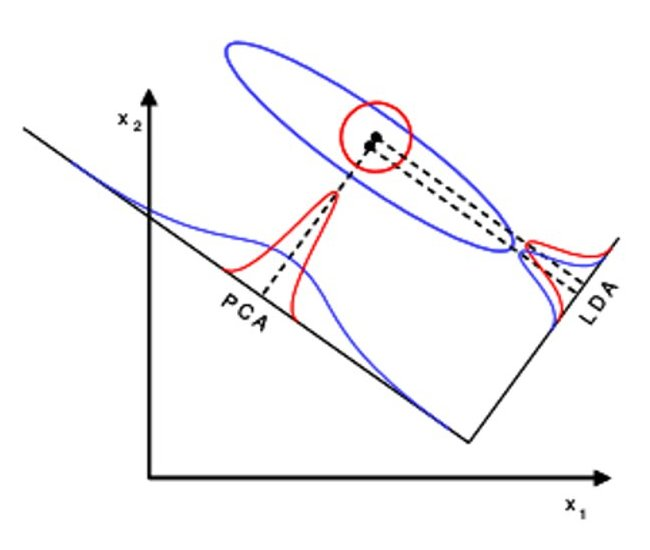
\includegraphics[scale=0.5]{img/limitation_lda}
  \caption{Two classes with similar means and different variances}
  \label{fig:lda-fail}
\end{figure}

Let's call the red class A, and the blue one B. The mean
of A and the mean of B are very close. There is just a slight
translation in one direction, and the LDA will project the data on the
side marked as ``LDA''. And obviously, this is not the good choice.

In the literature, there are several propositions to solve this problem.
The HLDA is one of them.

\subsection{HLDA}

\subsubsection{Differences between LDA and HLDA}

HLDA (Heteroscedastic Linear Discriminant Analysis) is another method to find a linear transformation mapping the problem space into a smaller one.

The HLDA finds the projection matrix A such that:
$$y = Ax$$
with $y$ a $p$-dimensions variable and $p < n$.\\

The purpose of the HLDA method is to release the homoscedasticiy constraint of the LDA, allowing different variances for each classes. The two assumptions made by the method are:

\begin{enumerate}
  \item The class distributions are $n$-dimensional Gaussian distributions.
  \item This space of size $n$ can be split into two subspaces of size $p$
    and $n - p$ (with $p < n$). The first one is different for all classes and contains meaningful information while the second one is the same for the whole dataset and contains only noise.
\end{enumerate}

The projection matrix A can then be rewritten following those assumptions:
$$A = \left [
  \begin{array}{c}
    A_p\\
    A_{n-p}
  \end{array}
\right ]
$$

it is also possible to find an expression for the mean and variance of each classes:
$$\mu_j =
\left [
  \begin{array}{c}
    \mu_{j,p}\\
    \mu_{0,(n-p)}
  \end{array}
\right ]
$$

$$\Sigma_j =
\left [
  \begin{array}{cc}
    \Sigma_j^p & 0\\
    0 & \Sigma_0^{(n-p)}\\
  \end{array}
\right ]
$$
Where $\mu_0$ and $\Sigma_0$ are supposed to be common to all classes.

Based on those definitions, it is possible to define a model representing the new dataset.

\subsubsection{HLDA Gaussian Model}

The Gaussian probability density function for this model is:
$$P(y_i) = \frac{\mid \theta \mid}{\sqrt{(2\pi)^n \mid \Sigma_{g(i)} \mid}}
e^{-\frac{1}{2} (y_i - \mu_{g(i)})^t \Sigma_{g(i)}^{-1} (y_i - \mu_{g(i)})}$$
With $g(i)$ the function associating each sample with its label.\\
The variables of the model are:
\begin{itemize}
  \item $A$: the projection matrix
  \item $\mu_j$ the mean of class $j$
  \item $\Sigma_j$ the covariance of class $j$
\end{itemize}

Note that $\mu_j$ and $\Sigma_j$ can depend on $A$ thus no analytical solution can be found (in contrast to the LDA method). In order to find estimators for those parameters Kumar\cite{kumar.1997} uses the maximum log-likelihood method and find two different solutions depending on the type of $\Sigma_j^p$.
To estimate the parameters found, a numerical-optimisation method is required.

\subsubsection{Full-rank $\Sigma_j^p$}

The Log-likelihood of the data $L_F = \sum\limits_{i = 1}^N log P(x_i)$ under the linear transformation $A$ and under the constrained Gaussian model assumption for each class is:
$$\begin{array}{cl}
  Log L_F(\mu_j, \Sigma_j, A; \{x_i\}) = & - \frac{1}{2} \sum\limits_{i = 1}^N\{(A^T x_i - \mu_{g(i)})^T\Sigma_{g(i)}^{-1}
  (A^T x_i - \mu_{g(i)}) \\
  & + Log((2\pi)^n|\Sigma_{g(i)}|)\} + Log|A|
\end{array}$$

Maximizing the Log-likelihood, knowing that there is a lot of parameters is very time consuming.
First, the values of the mean and variance parameters that maximize the log-likelihood with a fixed linear transformation $A$ are estimated.
These estimations are found by calculating the partial derivation of the log-likelihood equation. The maximum estimated values are the point where the partial derivatives are zero. \\
The mean and variance estimates are:
$$
\begin{array}{cc}
  \frac{\partial Log L_F(\mu_j, \Sigma_j, A; \{x_i\})}{\partial \mu_j} \Rightarrow \left \{
  \begin{array}{ccc}
    \hat\mu_j^p & = & A_p^T\bar{X_j} ,\; j = 1...J\\
    \hat\mu_0 & = & A_{n - p}^T\bar{X}
  \end{array}
  \right . \\
  \frac{\partial Log L_F(\mu_j, \Sigma_j, A; \{x_i\})}{\partial \Sigma_j} \Rightarrow \left \{
  \begin{array}{ccc}
    \hat\Sigma_j^p & = & A_p^T\bar{W_j}A_p, \; j = 1...J\\
    \hat\Sigma^{n - p} & = & A_{n - p}^T\bar{T}A_{n - p}
  \end{array}
  \right .
\end{array}$$

The substitution of this estimated values in the Log-likelihood equation give:
$$
\begin{array}{cl}
  Log L_F(A; \{x_i\}) = & \frac{-N n}{2}Log(2\pi)-\frac{N}{2}Log|(A_{n - p}^T\bar{T}A_{n - p})| \\
  & - \sum\limits_{j = 1}^J
  \frac{N_j}{2}Log|(A_p^T\bar{W_j}A_p)| \\
  & - \frac{1}{2}\sum\limits_{j = 1}^J\sum\limits_{g(i) = j} ((x_i - \bar{X_j})^TA_p(A_p^T\bar{W_j}A_p)^{-1}
  A_p^T(x_i - \bar{X_j})) \\
  & - \frac{1}{2}\sum\limits_{j = 1}^J\sum\limits_{g(i) = j} ((x_i - \bar{X})^TA_{n - p}(A_{n - p}^T\bar{T}A_{n - p})^{-1}
  A_{n - p}^T(x_i - \bar{X})) + N Log|A|
  \end{array}$$

The simplification of $L_F(A, \{x_i\})$ and it's maximization gives:
$$ \hat{A_F} = argmax_A\{-\frac{N}{2}Log|(A_{n - p}^T\bar{T}A_{n - p})| - \sum\limits_{j = 1}^J\frac{N_j}{2}Log|(A_p^T\bar{W_j}A_p)|
+ N Log|A|\}$$

$\hat{A_F}$ can be computed by a numerical-optimisation method.
To perform a dimension reduction transformation, we use only the first p columns of $\hat{A_F}$.

\subsubsection{Diagonal $\Sigma_j^p$}
Assuming the within-class covariance matrix to be diagonal, the calculus becomes easier.
From now, the matrix $\Sigma_j$ are supposed to be diagonal and their diagonal elements will be called $\{\sigma_j^1...\sigma_j^p,
\sigma^{p + 1}...\sigma^n\}$.
Note that when all $\Sigma_j$ are equals, the result is the same than the LDA one.

In this case, the log-likelihood of the data can be written as:
$$
\begin{array}{cl}
  Log L_D(\mu_j, \Sigma_j, A; \{x_i\}) = & -\frac{N n}{2} Log (2\pi) + N Log|A| - \frac{N}{2}\sum\limits_{k = p + 1}^n Log|\sigma^k| \\
  & - \sum\limits_{j = 1}^J \frac{N_j}{2} \sum\limits_{k = 1}^p Log|\sigma_j^k| - \frac{1}{2}\sum\limits_{j = 1}^J\sum\limits_{g(i) = j}
  \sum\limits_{k = 1}^p \frac{(\vec{A_k^T} - \mu_{j,k})^2}{\sigma_j^k} \\
  & + \frac{1}{2}\sum\limits_{j = 1}^J\sum\limits_{g(i) = j}
  \sum\limits_{k = p + 1}^p \frac{(\vec{A_k^T} - \mu_{0,k})^2}{\sigma^k}
\end{array}
$$

Using the same method than before to maximize $\mu_j$ and $\Sigma_j$

$$
\begin{array}{cc}
  \frac{\partial Log L_D(\mu_j, \Sigma_j, A; \{x_i\})}{\partial \mu_j} & \Rightarrow \left \{
  \begin{array}{ccc}
    \hat\mu_j^p & = & A_p^T\bar{X_j} ,\; j = 1...J\\
    \hat\mu_0 & = & A_{n - p}^T\bar{X}
  \end{array}
  \right . \\
  \frac{\partial Log L_D(\mu_j, \Sigma_j, A; \{x_i\})}{\partial \Sigma_j} & \Rightarrow \left \{
  \begin{array}{ccc}
    \hat\Sigma_j^p & = & Diag(A_p^T\bar{W_j}A_p), \; j = 1...J\\
    \hat\Sigma^{n - p} & = & Diag(A_{n - p}^T\bar{T}A_{n - p})
  \end{array}
  \right .
\end{array}
$$

After substitution in the main equation:
$$
\begin{array}{cl}
  Log L_D(A; \{x_i\}) = & - \frac{N n}{2} Log(2\pi) - \frac{N}{2} Log|Diag(A_{n - p}^T\bar{T}A_{n - p})| \\
  & - \sum\limits_{j = 1}{J}\frac{N_j}{2} Log|Diag(A_p^T\bar{W_j}A_p)| \\
  & - \frac{1}{2} \sum\limits_{j = 1}^J \sum\limits_{g(i) = j} ((x_i - \bar{X} )^T A_{n - p} Diag( A_{n - p}^T \bar{T} A_{n - p} )^-1 A_p^T(x_i - \bar{X}))\\
  & + N Log |A|
\end{array}
$$

After the simplification of $Log L_D(A; \{x_i\})$ and it's maximisation:
$$
\hat{A_D} = argmax_A\{-\frac{N}{2} Log|Diag(A_{n - p}^T \bar{T} A_{n - p})| - \sum\limits_{j = 1}^J \frac{N_j}{2} Log|Diag(A_{n - p}^T \bar{W_j} A_{n - p})| + N Log|A|\}
$$

$\hat{A_D}$ can be computed by a numerical-optimisation method.
To perform a dimension reduction transformation, we use only the first p columns of $\hat{A_D}$.

\subsubsection{Computing $\hat A$}

Now that the equations of $\hat{A_F}$ and $\hat{A_D}$ are defined, their values are calculated by numerical-optimization methods.
All methods that allow to find a maximum/minimum values in a function could work.
Kumar\cite{kumar.1997} uses a Gradient descent algorithm to perform the calculation.

\section{Variants of the HLDA}
\label{sec:variants}

There is several variants of the HLDA. We present them briefly.

First we will present a method which is a combination of the LDA and
the HDLA. In a second time, we present a method which allows to make our
computation faster.

\subsection{Smooth HLDA}
\label{sec:smooth-hlda}

If the HLDA works on a lot of classes, the estimation of the class
covariance becomes noisy. The LDA doesn't have this problem because
the within-class covariance matrix is the same for all the classes.

So, what is the solution when there is a lot of classes and the data
are not homoscedastics ? Burget\cite{burget.2004} presents a smooth
LDA. It is a combination of the LDA and the HLDA and it tries to get
the advantages of the two methods.

In this, we estimate the class covariance matrix as:

$$\breve\Sigma^{\left( j\right) }=\propto \hat\Sigma^{\left( j\right) } +\left( 1- \propto\right) \Sigma_{wc}$$

Where $\breve\Sigma^{\left( j\right) }$ is the smoothed estimated
covariance for the class $j$ used by the HLDA.
$\hat\Sigma^{\left(j\right) }$ is the covariance computed by the HLDA, and
$\Sigma_{wc}$ is the one computed by the LDA.

So it is clear that if $\propto$ is 1, the SHLDA is a HLDA, and if it
is equal to 1 it is a LDA.

\subsection{Diagonal Block HLDA}
\label{sec:db-hlda}

The HLDA is a very time consuming method. Performing it on real data set can be impossible as the data number of dimensions can be very high.
So an extension of the HLDA is to divide the research of $\hat{A}$ into independant subproblems.
This method is called Diagonal Block HLDA\cite{zhang2011}
$$
\hat{A} = \left [
\begin{array}{ccc}
\hat{A}^{1} \\
& \ddots \\
& & \hat{A}^{N}
\end{array}
\right ]
$$

With $\hat{A}^l, \; l = 1...N$ a subproblem to solve.
and $\hat{A}^l = argmax_{A_l}L^l (A^l; \{x_i\}^l)$

The equation for $L$ is:
$$
\begin{array}{cl}
  L(A; \{x_i\}) & = \sum\limits_{j = 1}^J \frac{I_j}{2} \sum\limits_{n = 1}^N Log \left ( \frac{|A^n|^2}{|Diag(A_{U^n}^n W_j^n (A_{U^n}^n)^T)||Diag(A_{M - U^n}^n T^n (A_{M - U^n}^n)^T)|} \right ) \\
  & = \sum\limits_{n = 1}^N L^n ( A^n; \{x_i^n\})
\end{array} 
$$

Each problem can be solved independantly.

%%% Local Variables:
%%% mode: latex
%%% TeX-master: "../hlda"
%%% End:

% ** Résultats
% *** Sur la base de Réda.
% *** Jolis graphiques.

\section{Results}
\label{sec:results}

The results presented in this section has been obtained on the MNIST database.
Each sample is encoded as a vector of 784 dimensions corresponding to a $28 \times 28$
pixels image. Each image represent a handwritten digit from 0 to 9, defining 9 different
classes.
The train dataset is composed of 60000 images and the test dataset of 10000.\\

The classifier used for the benchmark is simply a nearest mean classifier.
It associate to a sample the class that minimize the square distance between the class mean and
the sample mean.\\

{\bf Note:} Because of memory consumption issues, the HLDA algorithm is
run on smaller dimension samples. To do that, a PCA is applied to the samples keeping the
250 highest eigenvectors.

\subsection{HLDA parameters}

The HLDA method has a lot of parameters, some are linked to the dataset and some must be tuned
by the user.

\paragraph{Number of meaningful dimensions} The principal parameter to find is the number of dimension kept
by the algorithm, called $p$.

\begin{center}
  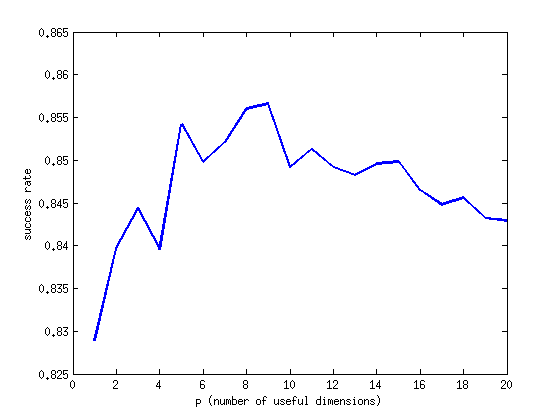
\includegraphics[scale=0.75]{img/bench-classes}
\end{center}

Interestingly the best classification ratio happens for $p = 9$ that
is exactly the number of dimensions kept by the LDA. Furthermore the farther we get from
it the worst the classification value get.

\section{Conclusions}
\label{sec:conclusions}

This is the end...



\bibliography{biblio}

\end{document}
